% !TEX program = xelatex
% Compile with any LaTeX environment that correctly renders this template.
\documentclass{article}
\usepackage[UTF8,scheme=plain,fontset=fandol]{ctex}
\usepackage{xcolor}
\usepackage{titleps}
\usepackage[letterpaper, margin=0.95in]{geometry}
\usepackage{url}
\usepackage{amsmath}
\usepackage{amssymb}
\usepackage{wrapfig}
\usepackage{float}
\usepackage{mathtools}
\usepackage{enumitem}
\usepackage{tabu}
\usepackage{parskip}
\usepackage{natbib}
\usepackage{listings}
\usepackage{tikz}
\usepackage{quiver}
\usepackage{graphicx}

\newcommand{\xb}{\mathbf{x}}
\newcommand{\yb}{\mathbf{y}}
\newcommand{\wb}{\mathbf{w}}
\newcommand{\Xb}{\mathbf{X}}
\newcommand{\Yb}{\mathbf{Y}}
\newcommand{\tr}{^T}
\newcommand{\hb}{\mathbf{h}}
\newcommand{\Hb}{\mathbf{H}}

\DeclareFontShape{OT1}{cmtt}{bx}{n}{<5><6><7><8><9><10><10.95><12><14.4><17.28><20.74><24.88>cmttb10}{}


\usepackage{forest}

\usepackage{hyperref}
\usepackage[color=red]{todonotes}
\usepackage{forest}
\definecolor{light-yellow}{HTML}{FFE5CC}

\usepackage{cleveref}

\newpagestyle{ruled}
{\sethead{RL2026fall / 95065}{增强学习}{Fall 2026}\headrule
  \setfoot{}{}{}}
\pagestyle{ruled}

\renewcommand\makeheadrule{\color{black}\rule[-.75\baselineskip]{\linewidth}{0.4pt}}
\renewcommand*\footnoterule{}

\begin{document}
\lstset{basicstyle = \ttfamily,columns=fullflexible,
backgroundcolor = \color{light-yellow}
}

\begin{centering}
    {\Large Assignment 2: Policy Gradients} \\
    \textbf{姓名：}\underline{潘昊辰} \qquad \textbf{学号：}\underline{523120910233} \\
    \vspace{.25cm}
    \textbf{提交截止日期见课程站点} \\
    \vspace{.15cm}
    提交入口：\url{https://oc.sjtu.edu.cn/courses/95065} \\
    \vspace{.15cm}
    \textbf{最终仅提交由本文件编译得到的 PDF 报告；无需提交代码、数据、实验日志或 TeX 源文件。}
\end{centering}

\setcounter{section}{0}

\section{Policy Gradients (CartPole Environment)}

In this section, you will evaluate the basic design choices in policy gradients:
trajectory-centric returns, reward-to-go, advantage normalization, and batch size.
To keep the workload manageable, we use four representative configurations.

\begin{lstlisting}[language=bash]
# 1. Vanilla policy gradient: trajectory-centric return, no normalization
python sjtuRL2026/scripts/run_hw2.py --env_name CartPole-v0 -n 100 -b 1000 \
    --exp_name cartpole_vanilla

# 2. Reward-to-go
python sjtuRL2026/scripts/run_hw2.py --env_name CartPole-v0 -n 100 -b 1000 -rtg \
    --exp_name cartpole_rtg

# 3. Reward-to-go + advantage normalization
python sjtuRL2026/scripts/run_hw2.py --env_name CartPole-v0 -n 100 -b 1000 -rtg -na \
    --exp_name cartpole_rtg_na

# 4. Reward-to-go + advantage normalization + larger batch size
python sjtuRL2026/scripts/run_hw2.py --env_name CartPole-v0 -n 100 -b 4000 -rtg -na \
    --exp_name cartpole_rtg_na_lb
\end{lstlisting}

Where:

\quad \verb|-n|: number of iterations

\quad \verb|-b|: batch size

\quad \verb|-rtg|: use reward-to-go

\quad \verb|-na|: use advantage normalization

\quad \verb|exp_name|: name of the experiment

\begin{itemize}
\item Create one graph comparing the learning curves
(average return vs. number of environment steps) for the four experiments above.

\textbf{For all plots in this assignment, the $x$-axis should be number of environment steps,
logged as} \verb|Train_EnvstepsSoFar|
\textbf{(\textit{not} number of policy gradient iterations).}

\item Answer the following questions briefly:
\begin{itemize}
\item Does reward-to-go improve performance compared with vanilla trajectory-centric returns?
\item Does advantage normalization help?
\item Does increasing the batch size from $1000$ to $4000$ improve stability or final performance?

\end{itemize}

\item Provide the exact command line configurations you used to run your experiments,
including any parameters changed from their defaults.

\item The best configuration should converge to a maximum score close to 200.
\end{itemize}

\newpage

\subsubsection*{实验图像与配置}
下图比较四组实验。横轴为 \verb|Train_EnvstepsSoFar|，纵轴为
\verb|Eval_AverageReturn|；左图放大前
$110{,}000$ 个环境步，右图展示完整训练过程。上方列出的四条命令即本实验的实际配置；
未列出的参数保持脚本默认值，包括随机种子 \verb|--seed 1|。每组训练 $100$ 次迭代，
前三组每次采集至少 $1{,}000$ 个环境步，最后一组至少采集 $4{,}000$ 个环境步。

\begin{figure}[H]
    \centering
    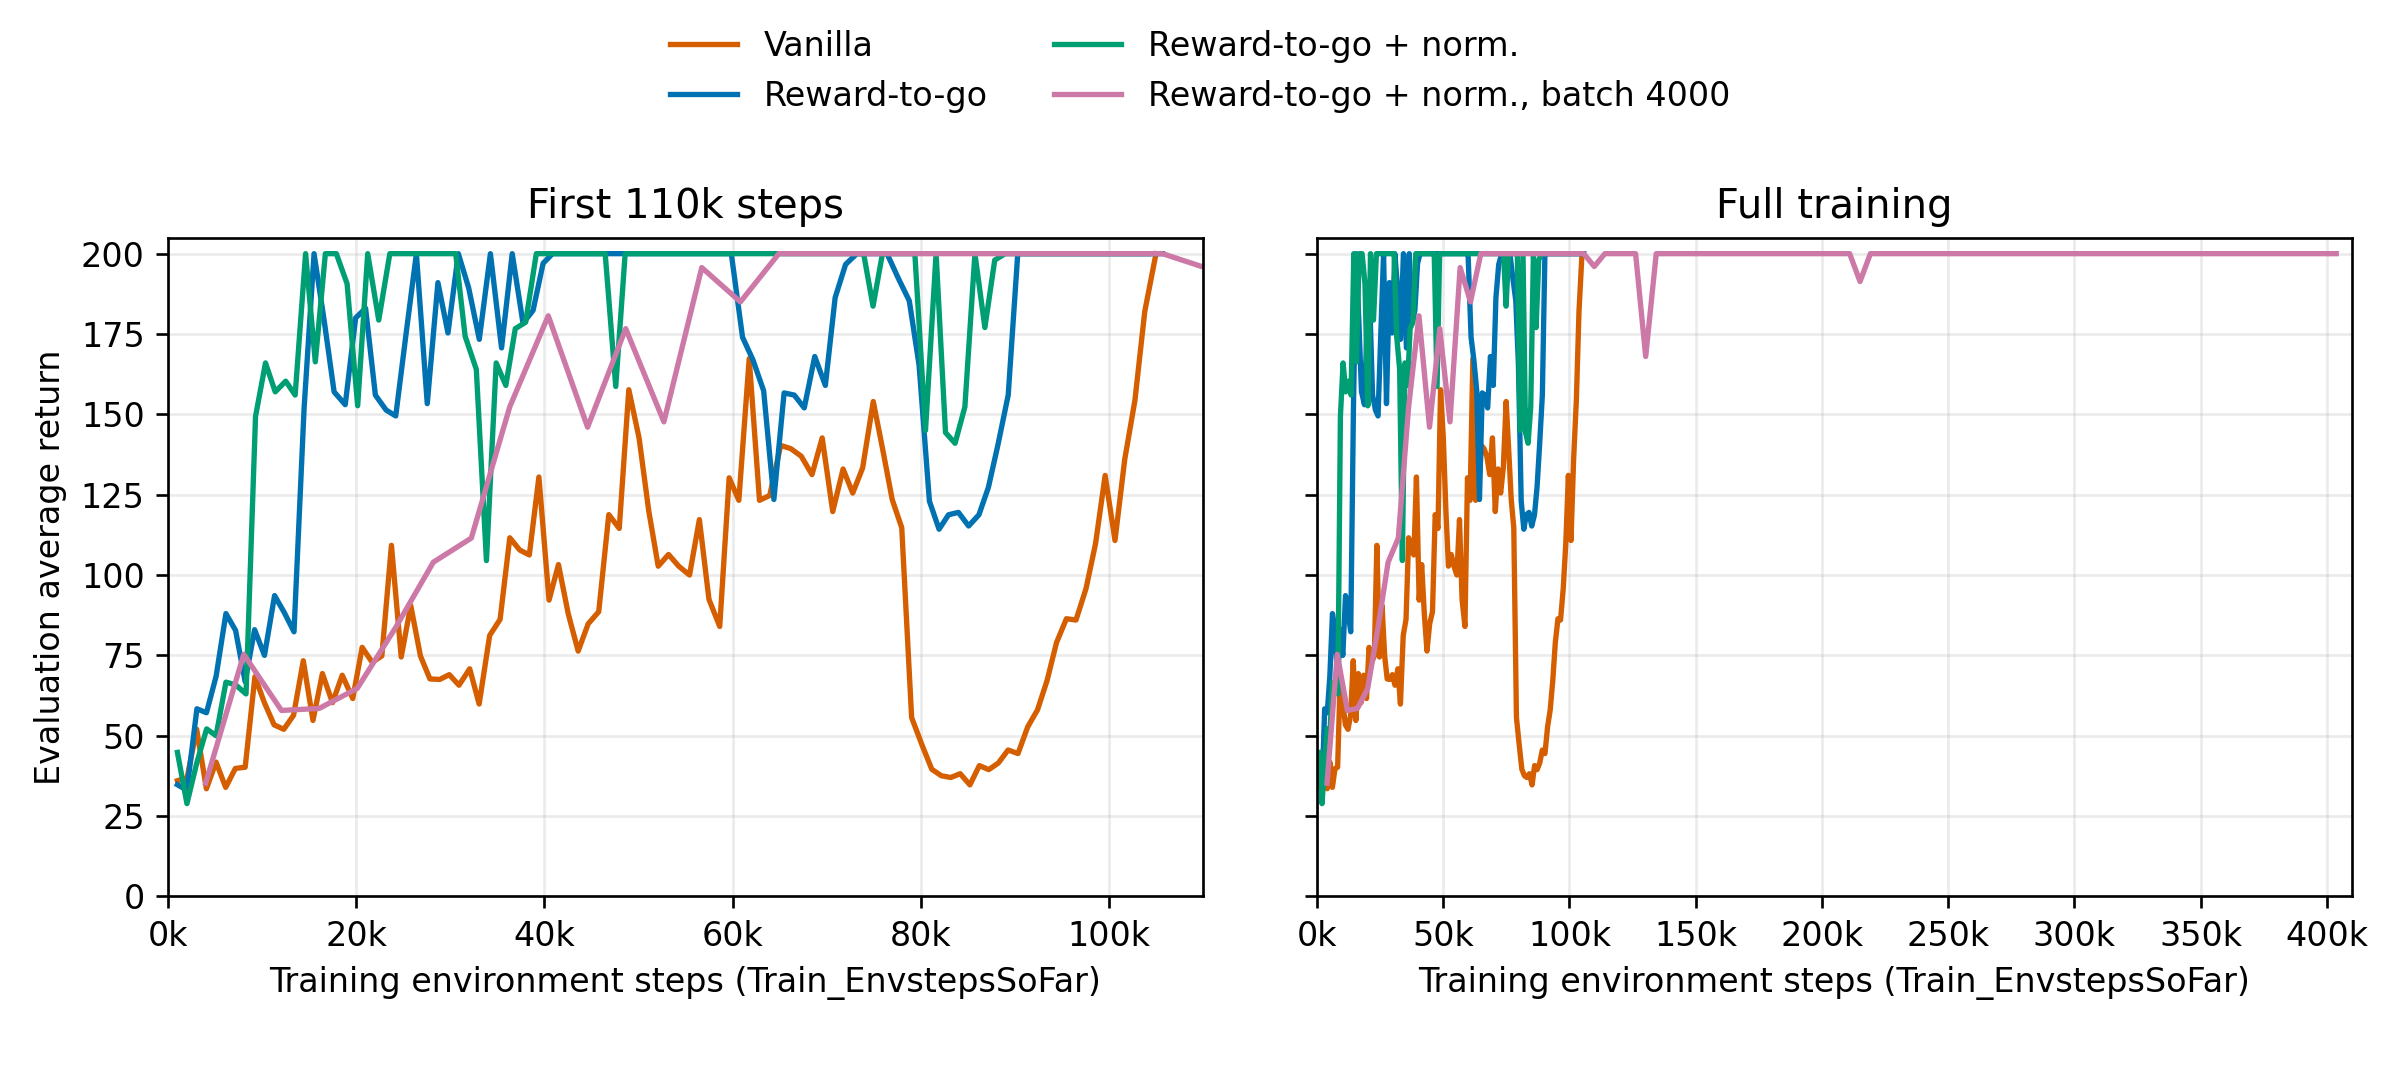
\includegraphics[width=\linewidth]{image/cartpole_learning_curves.png}
    \caption{CartPole-v0 上四种策略梯度配置的学习曲线}
\end{figure}

\paragraph{问题回答。}
\begin{enumerate}[label=(\arabic*)]
    \item Reward-to-go 改善了性能。在本次运行中，普通轨迹总回报方法
    首次达到 $190$ 分发生在约 $105{,}000$ 个环境步；reward-to-go 在约 $15{,}500$
    个环境步首次达到这一分数。普通方法后期仍有明显回落，最后 $10$ 次评估的平均分约为
    $129$；reward-to-go 对应的平均分为 $200$。
    \item 优势归一化有一定帮助。加入优势归一化后，首次达到
    $190$ 分所需的环境步数从约 $15{,}500$ 减少到约 $14{,}600$；两者最终均达到
    $200$ 分。这一差异来自单个随机种子的运行，不能据此断言对所有种子都更快。
    \item 批量大小增加后，大批量配置在达到高分后
    曲线较平稳，但首次达到 $190$ 分需要约 $56{,}700$ 个环境步；小批量的对应配置
    只需要约 $14{,}600$ 个环境步。两者最后 $10$ 次评估的平均分均为 $200$，
    因而本次运行未显示最终成绩的提升，且按环境交互次数衡量的学习速度更慢。
\end{enumerate}

\newpage

\section{Neural Network Baseline (HalfCheetah)}

You will now implement a value function as a state-dependent neural network baseline. This neural network will be trained in the update method of MLPPolicyPG along with the policy gradient update. We will train the baseline network for multiple gradient steps for each policy update, determined by the parameter \verb|baseline_gradient_steps|.

No baseline

\begin{lstlisting}[language=bash]
python sjtuRL2026/scripts/run_hw2.py --env_name HalfCheetah-v4 \
    -n 100 -b 5000 -rtg --discount 0.95 -lr 0.01 \
    --exp_name cheetah
\end{lstlisting}

Baseline

\begin{lstlisting}[language=bash]
python sjtuRL2026/scripts/run_hw2.py --env_name HalfCheetah-v4 \
    -n 100 -b 5000 -rtg --discount 0.95 -lr 0.01 \
    --use_baseline -blr 0.01 -bgs 5 --exp_name cheetah_baseline
\end{lstlisting}

You might notice that we omitted-na (normalize advantages). That’s because in reality, advantage normalization is a very powerful trick, and eliminates the need for a baseline most of the simple environments that we test in.


\begin{itemize}
    \item Plot a learning curve for the baseline loss.
    \item Plot a learning curve for the eval return. You should expect to achieve an average return over 300 for the baselined version.
    \item \textcolor{red}{(bonus)} Run another experiment with a decreased number of baseline gradient steps (\verb|-bgs|) and/or baseline learning rate (\verb|-blr|). How does this affect (a) the baseline learning curve and (b) the performance of the policy?
    \item \textbf{Optional:} Add \verb|-na| back to see how much it improves things. Also, set \verb|video_log_freq 10|, then open TensorBoard and go to the ``Images'' tab to see some videos of your HalfCheetah walking along!
\end{itemize}

\newpage
\subsubsection*{实验结果与分析}
上述两条命令为本实验的实际训练配置。两组均训练 $100$ 次迭代，每次采集
$5{,}000$ 个环境步，使用 reward-to-go、折扣因子 $0.95$ 和策略学习率 $0.01$；
第二组额外启用状态价值网络，价值网络学习率为 $0.01$，每轮更新 $5$ 次。


\begin{figure}[H]
    \centering
    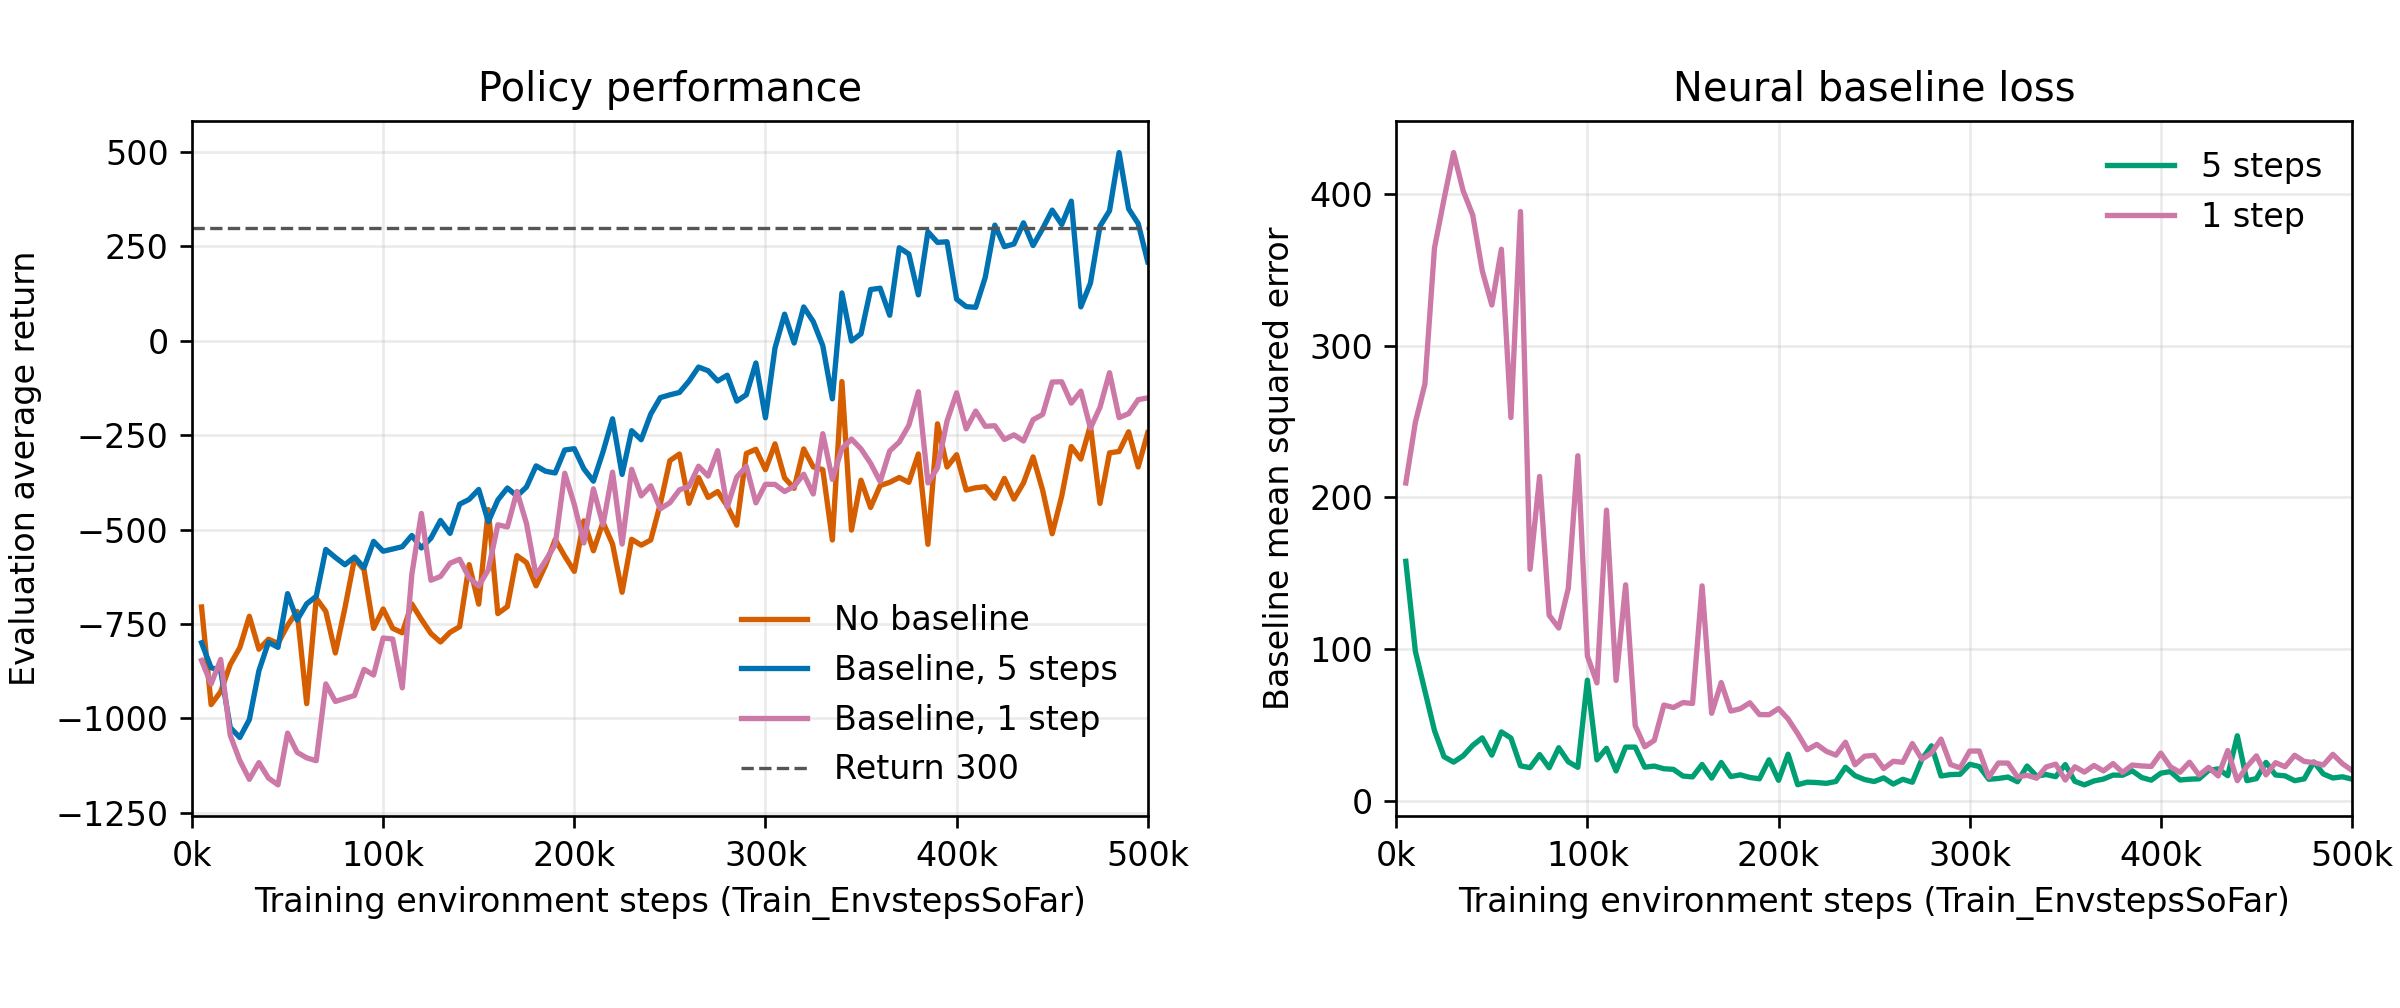
\includegraphics[width=\linewidth]{image/halfcheetah_baseline.png}
    \caption{HalfCheetah-v4 上无 baseline、每轮更新 $5$ 次与 $1$ 次 baseline 的对比。左图为评估平均回报，右图为 baseline 损失。}
\end{figure}

使用 baseline 时，价值网络的均方误差由首轮约 $158$ 降至最后一轮约 $14.5$，
中间仍有短暂波动。这表明网络逐渐拟合了回报目标，但不能把损失下降直接等同于策略
回报单调增加。未使用 baseline 的评估回报虽从约 $-705$ 提升，最后仍为约 $-244$，
整次运行的最高评估平均回报也只有约 $-108$。使用 baseline 后，回报从首轮约
$-800$ 提升，并多次超过 $300$，最高约 $499$，显示状态价值基线在本次运行中
显著改善了策略训练。

\par\vspace{\baselineskip}

保持其他参数与 baseline 实验一致，仅把每轮价值网络更新次数从 $5$ 降至 $1$：
\begin{lstlisting}[language=bash]
python sjtuRL2026/scripts/run_hw2.py --env_name HalfCheetah-v4 \
    -n 100 -b 5000 -rtg --discount 0.95 -lr 0.01 \
    --use_baseline -blr 0.01 -bgs 1 --exp_name cheetah_baseline_bgs1
\end{lstlisting}
在相同的默认随机种子下，\verb|-bgs 1| 的 baseline 损失从首轮约 $210$
降至最后一轮约 $20.3$，最后 $10$ 轮平均约 $24.7$；\verb|-bgs 5|
对应的最后 $10$ 轮平均约 $17.7$。图中一步更新的损失在训练前期更高、波动更明显。
策略方面，一步更新的最高评估平均回报约为 $-84.5$，最后一轮约为 $-151$，
最后 $10$ 轮平均约为 $-160$；五步更新的对应值为约 $499$、$209$ 和 $294$。
因此，本次运行中减少 baseline 更新次数削弱了价值估计的拟合效果，
并显著降低了最终策略表现。

\newpage\section{Generalized Advantage Estimation (LunarLander-v2) \textcolor{red}{(bonus)}}

You will now use the value function you previously implemented to implement a simplified version of GAE-$\lambda$. This will require filling in the remaining TODO section in \texttt{pg\_agent.py:estimate\_advantage}.

You will now use your implementation of policy gradient with generalized advantage estimation to learn a controller for a version of LunarLander-v2 with noisy actions. Search over $\lambda\in [0,0.95,0.98,0.99,1] $  to replace $<$todo$>$ below. Do not change any of the other hyperparameters (e.g. batch size, learning rate).

\begin{lstlisting}[language=bash]
for lambda in 0 0.95 0.98 0.99 1; do
  PYTHONPATH=.deps python sjtuRL2026/scripts/run_hw2.py \
    --env_name LunarLander-v2 --ep_len 1000 \
    --discount 0.99 -n 300 -l 3 -s 128 -b 2000 -lr 0.001 \
    --use_reward_to_go --use_baseline --gae_lambda "$lambda" \
    --exp_name "lunar_lander_lambda$lambda"
done
\end{lstlisting}

\begin{itemize}
    \item Provide a single plot with the learning curves for the \verb|LunarLander-v2| experiments that you tried. Describe in words how $\lambda$ affected task performance. The run with the best performance should achieve an average score close to 200 (180+).
    \item  Consider the parameter $\lambda$. What does $\lambda = 0$ correspond to? What about $\lambda = 1$? Relate this to the task performance in \verb|LunarLander-v2| in one or two sentences.
\end{itemize}

\newpage
\subsubsection*{参数$\lambda$的含义}
令 $\delta_t=r_t+\gamma(1-d_t)V(s_{t+1})-V(s_t)$，则优势的递推估计为
$\hat A_t=\delta_t+\gamma\lambda(1-d_t)\hat A_{t+1}$，其中 $d_t$ 表示轨迹终止。
$\lambda=0$ 时只保留单步 TD 误差，通常方差较低，但更依赖价值网络估计的准确性；
$\lambda=1$ 时累积至轨迹末端，在完整轨迹上等价于 Monte Carlo reward-to-go
减去 $V(s_t)$，通常偏差较低、方差较高。

\subsubsection*{实验结果与分析}
五组实验均按上方命令训练 $300$ 轮，仅改变 $\lambda$。\verb|PYTHONPATH=.deps|
用于加载本机所需的 Box2D 包，不改变训练超参数。图中的横轴为日志记录的
\verb|Train_EnvstepsSoFar|；浅色线为每轮原始评估回报，深色线为九点移动平均。

\begin{figure}[H]
    \centering
    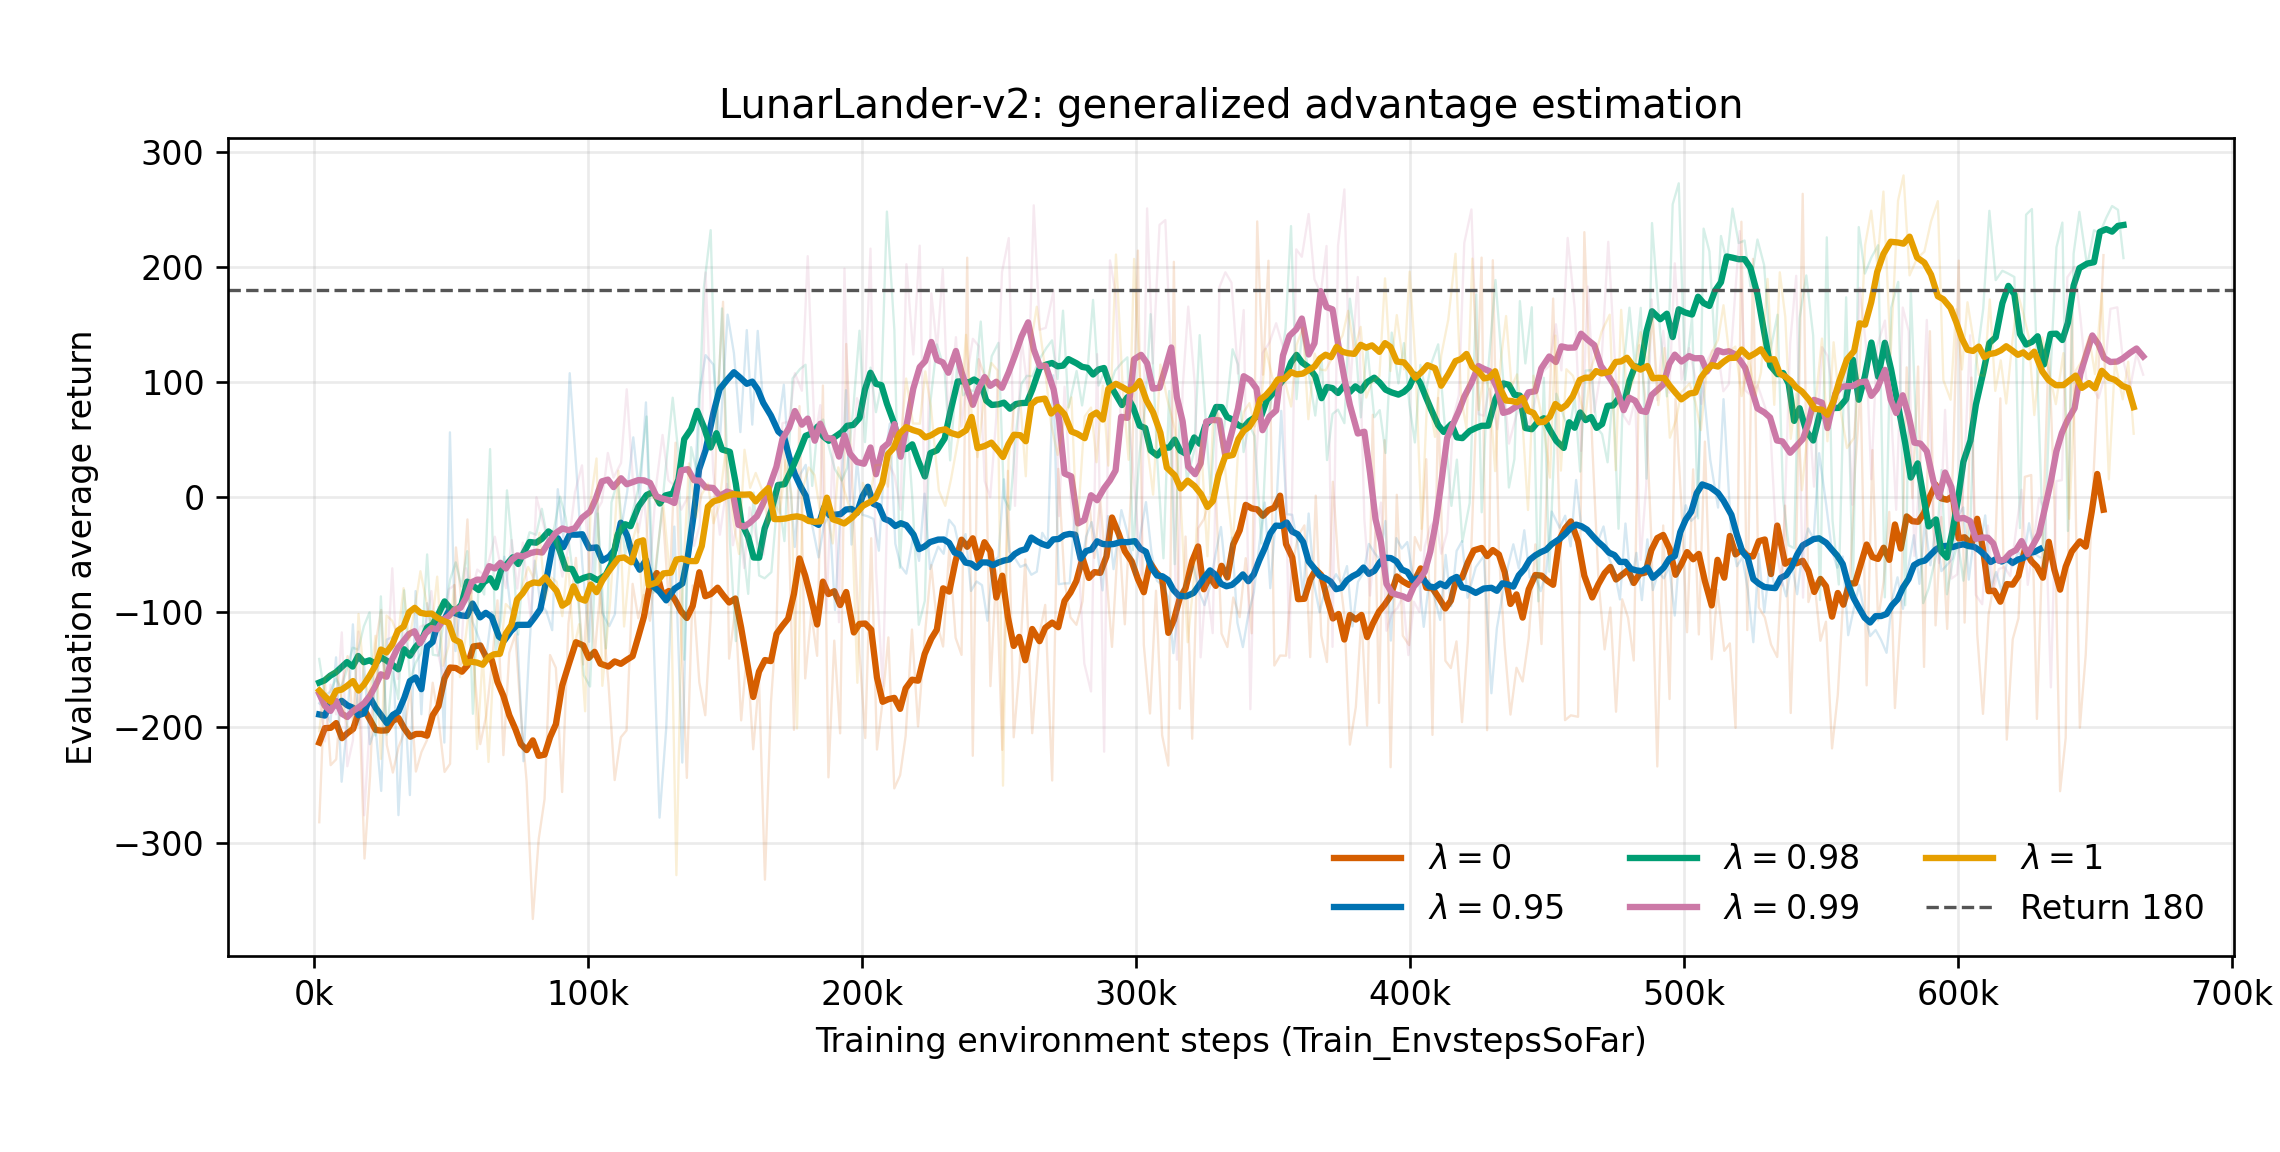
\includegraphics[width=\linewidth]{image/lunar_gae_lambda.png}
    \caption{LunarLander-v2 上五种 GAE $\lambda$ 的评估平均回报学习曲线。虚线标示 $180$ 分。}
\end{figure}

\begin{center}
\begin{tabular}{c|r|r}
$\lambda$ & 最后 $10$ 轮评估平均回报 & 单轮最高评估平均回报 \\
\hline
$0$ & $-21.4$ & $263.6$ \\
$0.95$ & $-56.5$ & $158.7$ \\
$0.98$ & $204.6$ & $272.7$ \\
$0.99$ & $116.4$ & $267.4$ \\
$1$ & $104.4$ & $279.6$ \\
\end{tabular}
\end{center}

本次运行中，$\lambda=0.98$ 的末段表现最好，最后 $10$ 轮评估平均回报约为
$205$，超过题目提出的 $180$ 分目标。$\lambda=0$ 虽曾单轮达到约 $264$ 分，
但末段均值为负，说明其表现不稳定；$\lambda=0.95$ 始终未达到 $180$ 分。
$\lambda=0.99$ 和 $1$ 均曾达到较高峰值，但最后 $10$ 轮均值分别约为 $116$
和 $104$。

\newpage\section{Hyperparameter Tuning (InvertedPendulum) \textcolor{red}{(bonus)}}

First, train a policy for the inverted pendulum problem without GAE and with otherwise default settings. Use five different seeds to get a good estimate of average performance

\begin{lstlisting}[language=bash]
for ($seed = 1; $seed -le 5; $seed++) {
  python sjtuRL2026/scripts/run_hw2.py --env_name InvertedPendulum-v4 -n 100 \
    --exp_name "pendulum_default_s$seed" \
    -rtg --use_baseline -na \
    --batch_size 5000 \
    --seed $seed
}
\end{lstlisting}

Your task is to tune hyperparameters so that your implementation reaches maximum performance (score of 1000) in fewer environment steps than these default settings (note: this is not the same as minimizing number of policy gradient iterations: one policy gradient iteration corresponds to batch size environment steps). Try and find hyperparameters that reach a score of 1000 in as few steps as possible !

\begin{enumerate}
    \item Provide a set of hyperparameters that achieve high return on \verb|InvertedPendulum-v4| in as few environment steps as possible.
    \item Show learning curves for the average returns with your hyperparameters and with the default settings, with environment steps on the $x$-axis. Returns should be averaged over 5 seeds.
\end{enumerate}

\newpage

\textbf{实验设置与调参结果。}\par

在 \texttt{InvertedPendulum-v4} 上均使用
reward-to-go、价值基线和优势标准化，不使用 GAE。比较五个随机种子
（$1,2,3,4,5$）的评估平均回报。默认组采用题目指定的 batch size
$5000$、策略学习率 $0.005$，训练 $100$ 轮；调参组把 batch size
降至 $500$、策略学习率升至 $0.01$，训练 $200$ 轮。其余参数均保持脚本默认值，
包括基线学习率 $0.005$、每轮基线更新 $5$ 步、折扣因子 $1$、
两层各 $64$ 个神经元。

运行的命令如下（两组分别执行）：
\begin{lstlisting}[language=bash]
for seed in 1 2 3 4 5; do
  python sjtuRL2026/scripts/run_hw2.py \
    --env_name InvertedPendulum-v4 -n 100 \
    --exp_name "pendulum_default_s${seed}" \
    -rtg --use_baseline -na --batch_size 5000 --seed "${seed}"
done

for seed in 1 2 3 4 5; do
  python sjtuRL2026/scripts/run_hw2.py \
    --env_name InvertedPendulum-v4 -n 200 \
    --exp_name "pendulum_tune_b500_lr01_s${seed}" \
    -rtg --use_baseline -na --batch_size 500 \
    --learning_rate 0.01 --seed "${seed}"
done
\end{lstlisting}

\begin{figure}[H]
  \centering
  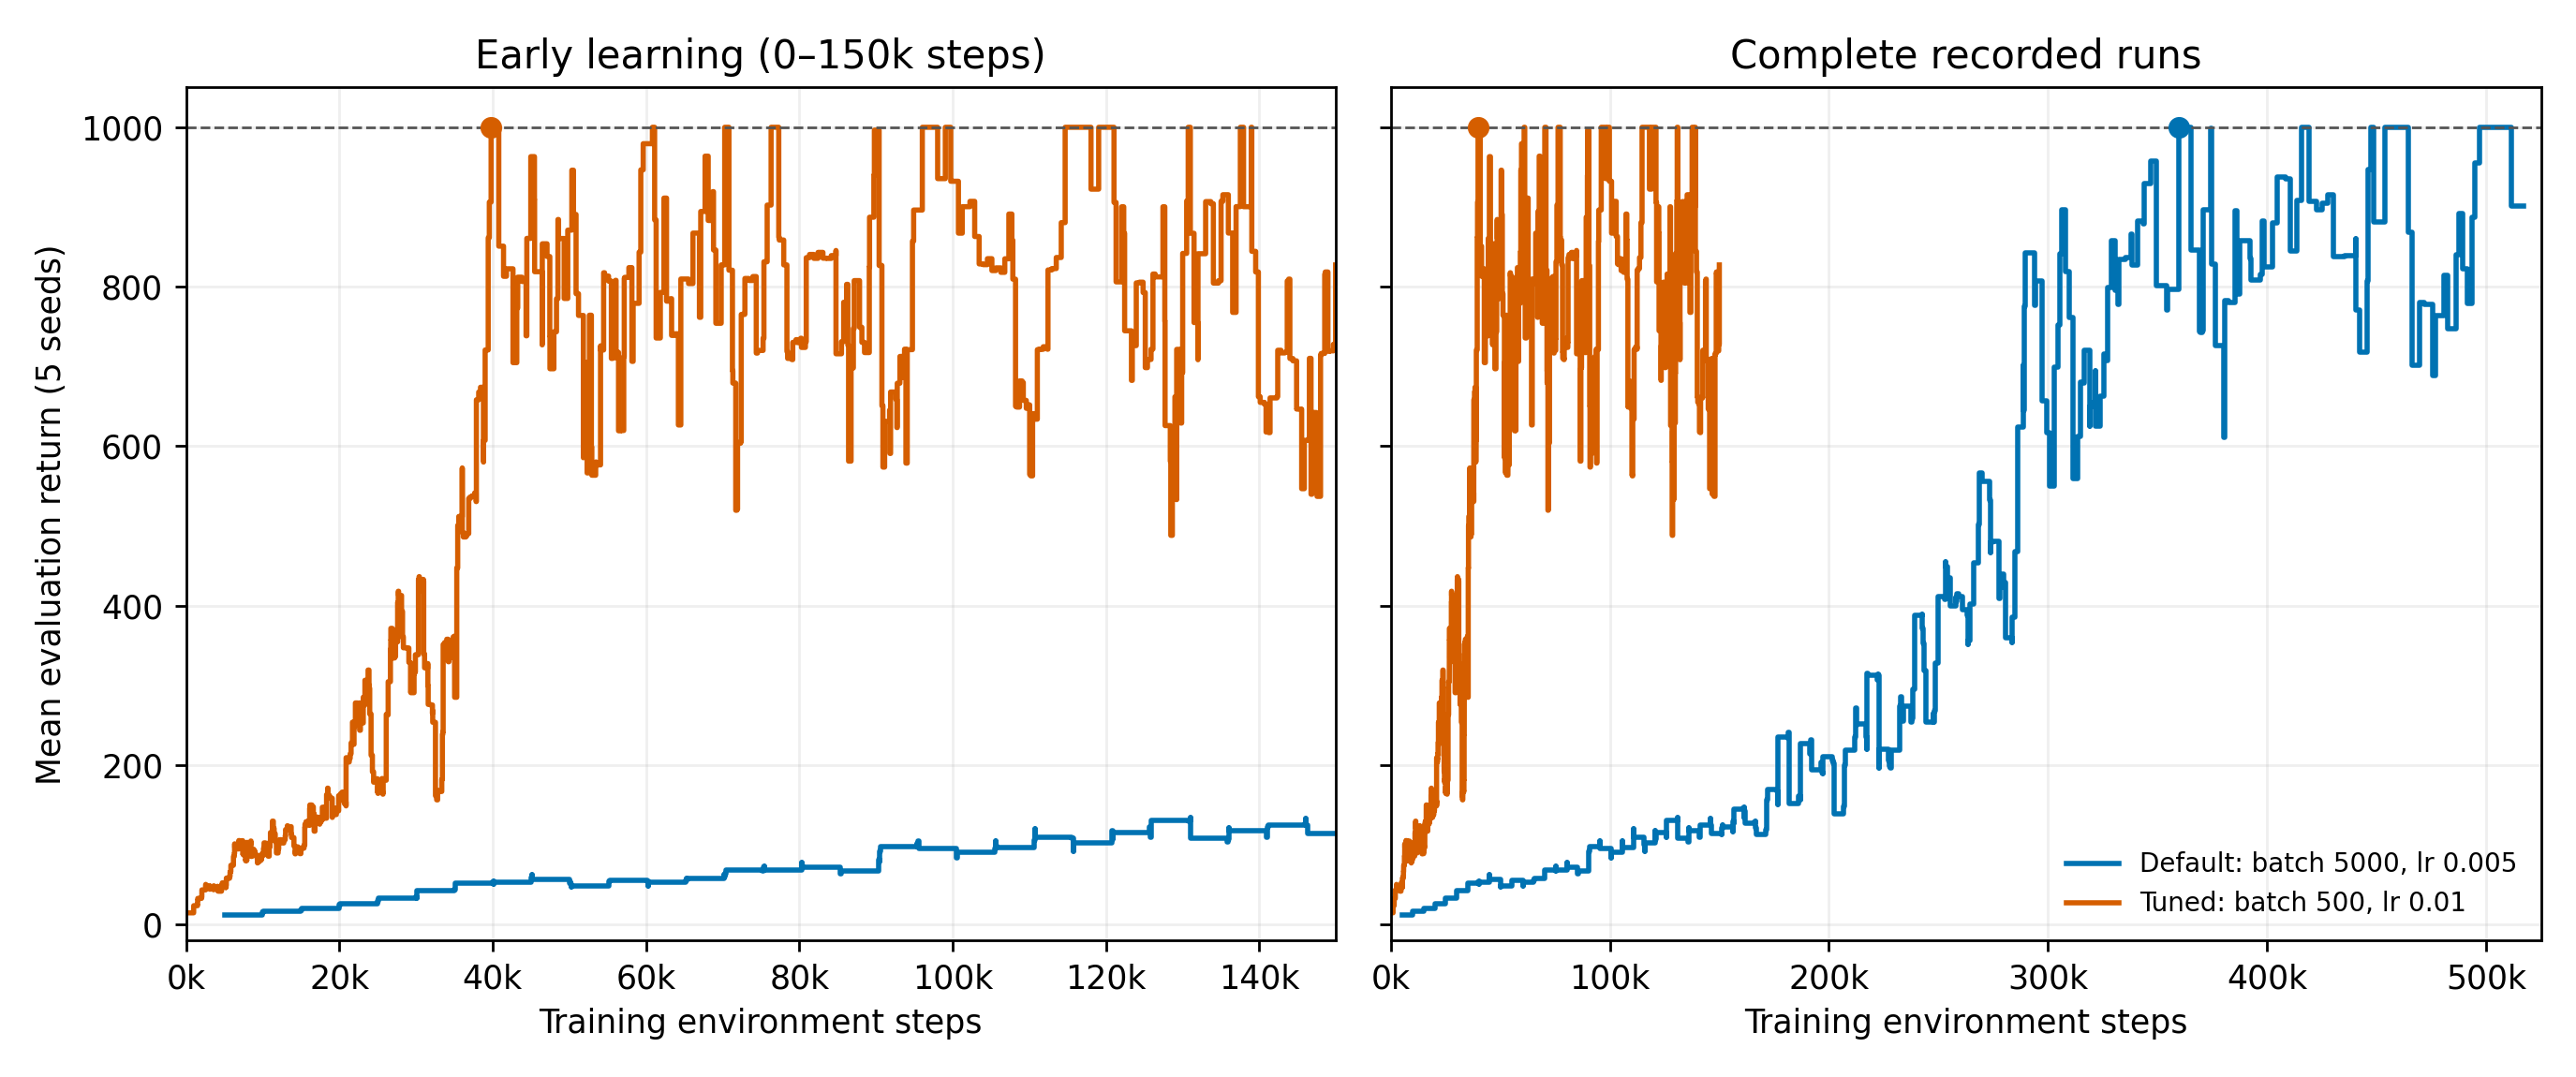
\includegraphics[width=\linewidth]{image/pendulum_tuning.png}
  \caption{InvertedPendulum-v4 problem默认配置与调参配置的五种子平均评估回报。横轴取日志中的
  \texttt{Train\_EnvstepsSoFar}；按各自记录的实际环境步数对齐，并沿用上一次
  评估值计算五种子均值。左图放大前 $15$ 万步，右图展示完整记录区间。
  圆点标出五种子均值首次达到 $1000$ 分的位置；曲线未平滑。}
  \label{fig:pendulum-tuning}
\end{figure}

\begin{center}
\begin{tabular}{lrrr}
\hline
配置 & Batch size & 策略学习率 & 五种子均值首次达 $1000$ 的步数 \\
\hline
默认 & $5000$ & $0.005$ & $359{,}750$ \\
调参 & $500$ & $0.01$ & $39{,}803$ \\
\hline
\end{tabular}
\end{center}

调参配置首次达到五种子平均满分时，比默认配置少用了约 $88.9\%$ 的
训练环境步数（约快 $9.0$ 倍）。

\newpage

\section{提交说明：仅提交 PDF 报告}

请把实验图表、命令配置和文字答案填写到 \texttt{hw2\_template.tex} 中，并使用任意能够正确编译本模板的 LaTeX 环境生成 PDF。最终文件应为 \texttt{hw2\_template.pdf}。

\textbf{课程平台只需上传填写完整且能够正常打开的 PDF 报告。无需上传 Python 代码、实验数据、日志、模型文件、TeX 源文件或 ZIP 压缩包。} 代码和实验输出仅用于完成实验与生成报告内容，请自行保留。

提交前请逐页检查 PDF，确认图表、公式、命令和答案均显示完整。提交入口：\url{https://oc.sjtu.edu.cn/courses/95065}。截止日期以课程平台通知为准。

\end{document}
